\documentclass{amsbook}
\usepackage{graphicx} % Required for inserting images
\usepackage{float}
\usepackage[colorlinks=true,linkcolor=blue]{hyperref}
\usepackage{amssymb}
\usepackage{enumerate}
\usepackage{mathtools}
\usepackage{tikz}
\usepackage[answerdelayed]{exercise}
\usepackage{floatflt}
\usepackage{multicol}
\usepackage{subcaption}
\usepackage{tikz}
\usepackage{tkz-euclide}
\usetikzlibrary{trees}

\usepackage[backend=biber,style=alphabetic,sorting=ynt]{biblatex}
\addbibresource{calc.bib}

\setlength{\parindent}{0pt}
\setlength{\listparindent}{0pt}
\renewcommand{\ExerciseHeaderTitle}{\quad\ExerciseTitle}
\renewcommand{\AnswerHeader}{\medskip\centerline{\emph{\ExerciseName\ \ExerciseHeaderNB} \smallskip}}
\renewcommand{\ExerciseHeader}{\medskip\ExerciseHeaderDifficulty{\emph{\ExerciseName\ \ExerciseHeaderNB\ExerciseHeaderTitle} \newline}}
\renewcommand{\QuestionNB}{(\alph{Question})\ }
\renewcommand{\Re}{\operatorname{Re}}
\renewcommand{\Im}{\operatorname{Im}}


%%%%%%%%%%

\begin{document}

\title{Calculus Problem Book:\\
    \Large Form V and Form VI}


\author{S. Chu}

\maketitle
\tableofcontents
\chapter*{Preface}
The following short booklet contains a collection of problems with solutions that roughly follow the topics typically covered in the calculus sequence for Form V and Form VI mathematics classes at Ethical Culture Fieldston School. The hope is to provide a book of problems of varying difficulty that will provide non-routine exercises for students learning Calculus, as well as to record general themes and approaches to tackling these types of problems. Ideally these problems can be useful to all courses that cover these topics. Problems are roughly categorized by difficulty level and notated via *, **, or *** in increasing difficulty.\\ \\
At the end of text we have included several longer problems that allow students to tackle more complex problems that often synthesize material from several areas as well as giving students a look at some applications of Calculus to other fields. We have adopted problems from memory, and from years of working with the material. The following references were consulted for problems as well as other considerations such as narrative structure in introducing various topics and thematic development of the material. \cite{mcirc}, \cite{aops}, \textcite{spk}, [more later].
\chapter{Functions and Other Miscellaneous Content}

\section{Set Notation and Numbers}
\begin{Exercise}[title={Sets, Unions and Intersections}, difficulty = 0, label= 1b1]
	Set $A \subset B$ iff every element of $A$ in also in $B$. Set $A \supset B$ iff every element of $B$ is also in $A$ and two sets are equal iff both $A\supset B$ and $A\subset B$. 
	\begin{enumerate}
		\item If $A \subset B$ then what is the set $A \cap B$?\\
		\item If $A \subset B$ then what is the set $A \cup B$?\\
		\item If $A \cup B = B$, give an argument that explains why $A \subset B$.
	\end{enumerate}
	
\end{Exercise}

\begin{Exercise}[title={Complements}, difficulty=0, label = 1b2]
	Given a set $A$, and a set $B$ we can define the complement of that set, $A^c$ or sometimes: $\overline{A}$, $A'$, or $B-A$, as the elements in $B$ but not in $A$.  Notice $A^c, A'$ and $\overline{A}$ do not reference the set $B$ and are often used when no confusion can arise or there is some all encompassing universal set $U$ that contains $A$.
		\begin{enumerate}
			\item Given a universal set $U$ and $A, B$ contained in $U$. Show that $ (A\cap B)^c =A^c \cup B^c$ by first showing that $(A \cap B)^c \subset A^c \cup B^c$. Then show that $(A \cap B)^c \supset A^c \cup B^c$. This property is often called DeMorgan's Law.
			\item Describe the elements that are contained in the set $(A-B) \cup (B-A)$. This set is called the symmetric difference of A and B, or $A \Delta B$.
		\end{enumerate}

\end{Exercise}

\begin{Exercise}[title={Working with Sets}, difficulty=2, label=1b3]

	In the previous problem we defined the symmetric difference. The following exercises will work through some properties of this operation on sets. Recall that to show two sets $A, B$ are equal you must show that $A \subset B$ ie. every element is $A$ is also in $B$, as well as that $B \subset A$, ie. every element of $B$ is also in $A$.
	\begin{enumerate}
		\item Show that $(A-B) \cup (B-A) = (A \cup B) - (A\cap B)$ as sets. These are two different ways to think about the set that is the symmetric difference of two sets $A \Delta B$. Let $A, B$ be arbitrary sets.
		\item Show that $A \Delta B = B \Delta A$ by showing that every element in the set on the left is in the set on the right and vice versa.
		\item Show that $A \Delta \varnothing  = A$. Where $\varnothing$ is the empty set.
		\item Show that $A \Delta A = \varnothing$.
		
		
	\end{enumerate}

\end{Exercise}

%%%%
%%%%

\section{Working with Inequalities}

%%%%
%%%%

\section{Polynomials}


%%

\begin{Exercise}[title={Polynomials I}, difficulty=0 , label=1a1 ]
	Let $f(x)=x^2-3$ and $g(x)=x^3-2x$. Both $f$ and $g$ are polynomials. You can form new polynomials by adding, subtracting, multiplying, and composing. 
        \begin{enumerate}
            \item Find $(f+g)(x)$
            \item Find $(f-2g)(x)$
            \item Find $(f\cdot g)(x)$
            \item Find $f \circ g)(x)$
            \item Explain why $(f/g)(x)$ is not a polynomial.
        \end{enumerate}

	\hfill \emph{solution} \refAnswer{1a1}
\end{Exercise}

\begin{Answer}[ref={1a1}]
	blah blah
\end{Answer}

\begin{Exercise}[title={Defining Polynomials}, difficulty=1, label=1a2]
A polynomial $f$ has the general form $f(x)=a_0+a_1 x + a_2 x^2 + \ldots +a_{n-1}x^{n-1} + a_nx^n$, where $n \in \mathbb{Z}$ and $a_i \in \mathbb{R}$. Show that adding, subtracting, or multiplying two polynomials always results in a polynomial. Explain why this is not the case for division.

    \hfill \emph{solution} \refAnswer{1a2}
\end{Exercise}

\begin{Answer}[ref={1a2}]
    The expression $A \subset B$ is read, the set $A$ is contained in the set $B$. Whereas the expression $A \supset B$ is read the set $A$ contains the set $B$.
    \begin{enumerate}
        \item $\mathbb{Z}\supset \mathbb{N}$
        \item $\mathbb{R}\supset \mathbb{Q}$
        \item $\mathbb{N} \subset \mathbb{Q}$
    \end{enumerate}
\end{Answer}

\begin{Exercise}[title={Polynomials II}, difficulty =0, label=1a3]
   A function $f$ is even if and only if $f(x)=f(-x)$ for all $x$ in its domain. A function is odd if and only if $f(-x)= - f(x)$ for all $x$ in its domain.
   	\begin{enumerate}
   		\item Give an example of an even polynomial.
   		\item Give an example of an odd polynomial.
   	\end{enumerate}
\end{Exercise}

%%%%%%%%%%%%%%%%%%%%%%%%%%%%%%%%%%%%%%%%


\section{Trigonometric Functions}

%%%%%%

\section{Miscellaneous}

%%%%%%%%%%%%%%%%%%
%%%%%%%%%%%%%%%%%%
\chapter{Limits and Continuity}


\section{Intuitive Notion}

\section{Epsilon and Delta}

\begin{Exercise}[title={Dirichlet Function}, difficulty=1 , label=2b1 ]
	The Dirichlet function $D$ is define as $D(x)=\left\{\begin{array}{c l} 1 & x\in \mathbb{Q} \\ 0 & \mbox{otherwise}\end{array} \right.$. Two sets of numbers are \emph{not seperable} if it is impossible to find an open interval around an element from one set that contains only elements from that set and not the other. Rational numbers and irrational numbers are not separable. Use this  to argue that $\lim \limits_{x\to a} D(x)$ does not exist for any value of $a$.
	\hfill \emph{solution} \refAnswer{2b1}
\end{Exercise}

\begin{Answer}[ref={2c1}]
	blah blah
\end{Answer}

\begin{Exercise}[title={A Strange Function}, difficulty=3, label=2b2]
	Let $f(x)=\left\{ \begin{array}{c c} 0 & \quad x \in \mbox{ irrational} \cap [0,1] \\
	\frac{1}{q} & \quad x=\frac{p}{q} \mbox{ in lowest terms}, 0<x<1 \end{array} \right.$ \\[.5cm]
	For any $a \in [0,1]$, find the $\lim \limits_{x \to a} f(x)$. Show the limit you calculated is in fact the limit by giving an appropriate delta neighborhood for a given $\epsilon >0$. \textcite{spk}

\hfill \emph{solution} \refAnswer{2b2}
\end{Exercise}

\begin{Answer}[ref={2b2}]
  First make a sketch of the function.
\end{Answer}

\section{Continuity}
\begin{Exercise}[title={A Bounded Function around Zero}, difficulty=1 , label=2c1 ]
	Let $f: \mathbb{R} \to \mathbb{R}$ be a function such that $|f(x)| \leq |x| $ for all $x$ in the domain of $f$.  Prove that $f$ is continuous at $x=0$.

	\hfill \emph{solution} \refAnswer{2c1}
\end{Exercise}

\begin{Answer}[ref={2c1}]
	blah blah
\end{Answer}

\begin{Exercise}[title={Some Points Don't Move That Much}, difficulty=1 , label=2c2 ]
	Let $f:[0,1] \to [0,1]$ be a function such that $|f(x)| \leq |x| $ for all $x$ in the domain of $f$.  Prove that $f$ is continuous at $x=0$.

	\hfill \emph{solution} \refAnswer{2c2}
\end{Exercise}

\begin{Answer}[ref={2c2}]
	blah blah
\end{Answer}




\section{Intermediate Value Theorem}
\begin{Exercise}[title={Degree 3 Polynomial with Real Roots}, difficulty=1, label=2d1]
Let $f(x)=(x-a)(x-b)+(x-b)(x-c)+(x-a)(x-c)$ where $a,b,c$ are distinct real numbers. Prove that $f$ must have 3 real distinct zeroes.


\end{Exercise}

\begin{Answer}[ref={2d1}]
	Look at $f(a)$, $f(b)$ and $f(c)$.  Since $a,b,$ and $c$ are distinct we can assume they are ordered $a<b<c$, this will then put you in a position to apply IVT.
\end{Answer}

\begin{Exercise}[title={Fixed points}, difficulty=1, label=2d2]
Let $f$ be a continous function from the unit interval to itself. $f:[0,1] \to [0,1]$. Show that $f$ must have at least one fixed point $x_0$.  In other words,  $f(x_0)=x_0$.

\end{Exercise}

\begin{Exercise}[title={Antipodes}, difficulty = 2, label=2d3]
Two points on a sphere are antipodal if the line connecting them passes through the center of the sphere. They are 'directly opposite' one another, or maximally distant from one another while still being on the sphere. 
	\begin{enumerate}
		\item If you assume that the earth is a sphere and that temperature varies continuously from point to point on the earth, show that there must be a pair of antipodal points that are the same temperature at a given moment in time.\\
		\item If we also assume that air pressure varies continuously across the earth, show that there must be a pair of antipodal points on the surface of the earth that have the same temperature and air pressure at a given moment in time. \\
	\end{enumerate}

\end{Exercise}

\begin{Answer}[ref={2d3}]
	Both require looking at the difference in the function evaluated at a pair of antipodes.
\end{Answer}

%%%%%%%%%%%
%%%%%%%%%%5i

\chapter{The Derivative}

\section{Limit Definition and Properties of the Derivative}
\begin{Exercise}[title={Introducing a Discontinuity}, difficulty=0, label=3a1]
Let $f(x)=|x|$. Use the limit definition of the derivative to show that $f'(x)=\dfrac{|x|}{x}$. Show using the definition of continuity how the derivative 

\end{Exercise}

\begin{Answer}[ref={3a1}]
    
\end{Answer}

\section{Tangent Line Problem}

\section{Higher Order Derivatives}

\section{Power Rule and others}
\begin{Exercise}[title={Unit Circle and Sine}, difficulty=1 , label= 3d1]
	Let $P=(\cos \theta,\sin \theta)$. Use similar triangles to calculate an approximation for $\dfrac{\Delta y}{\Delta \theta}$ and explain how this shows what the derivative of $f(x)=\sin (x)$ is.  Do the same for $g(x)=\cos(x)$ by looking at $\dfrac{\Delta x}{\Delta \theta}$.
		\begin{figure}[H]
			\centering
			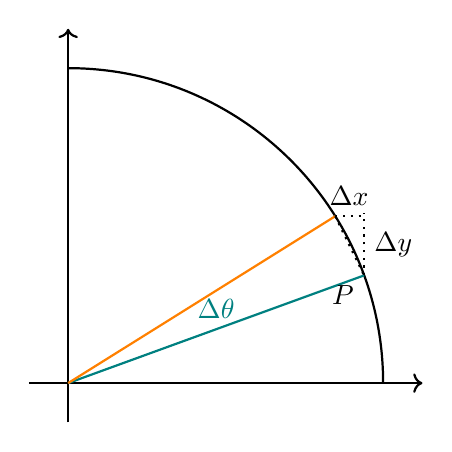
\begin{tikzpicture}
			\draw[thick](4,0)arc(0:90:4);
			\draw[thick,->](-.5,0)--(4.5,0);
			\draw[thick,->](0,-.5)--(0,4.5);
			\tkzDefPoint(4,0){A}
			\tkzDefPoint(0,0){B}
			\tkzDefPointBy[rotation=center B angle 20](A) \tkzGetPoint{C}
			\draw[thick, color=teal](B)--(C) node[midway, above]{$\Delta \theta$};
			\tkzDefPointBy[rotation=center B angle 12](C) \tkzGetPoint{D}
			\draw[thick, color= orange](B)--(D);
			\draw[thick,dotted](C)--+(0,.79) node[midway,right]{$\Delta y$};
			\draw[thick,dotted](D)--+(.35,0) node[midway, above]{$\Delta x$};
			\draw[thick,dotted](D)--(C) node[at end, below left]{$P$};
			\end{tikzpicture}
		\end{figure}

	\hfill \emph{solution} \refAnswer{3d1}
\end{Exercise}

\begin{Answer}[ref={3d1}]
	blah blah
\end{Answer}

\section{Implicit Differentiation}

%%%%%%%%%%
%%%%%%%%%%%

\chapter{Applications of the Derivative}

\section{Related Rates}

\section{Mean Value Theorem}

\section{Maximums and Minimums}

\section{Optimization and Graphing}

%%%%%%%%%
%%%%%%%%%

\chapter{The Integral}
\section{Series}

\section{Riemann Sums}


\section{Riemann Integrable}


\section{Properties of the Integral}


%%%%%%%%%%%
%%%%%%%%%%%%

\chapter{The Fundamental Theorem of Calculus}

\section{Anti-Derivatives}

\section{FTC part I}

\section{FTC part 2}

\section{Functions Defined by an Integral}

\section{Integral as Accumulator}

\section{U Substitution}

\section{Probability Distributions}

%%%%%%%%%%%%
%%%%%%%%%%%

\chapter{Logarithms, Exponentials, and Inverses}

\section{Logarithms}

\section{Inverse Functions}

\section{Exponentials}

\section{Inverse Trigonometric Functions}

\section{Hyperbolic Trigonometric Functions}



%%%%%%%%%%
%%%%%%%%%%%%

\chapter{Methods of Integration}


\section{Integration by Parts}

\section{Method of Partial Fractions}

\section{Trigonometric Substitutions}

\section{Improper Integrals}

%%%%%%%%%
%%%%%%%%%

\chapter{Differential Equations}
\section{Slope Fields and Euler's Method}

\section{Separation of Variables}

\section{Modeling}

\section{Logistic Growth}

\section{Systems of Differential Equations}

\section{Reduce 2nd order equations to two 1st order equations}


%%%%%%%%%%
%%%%%%%%%%

\chapter{More Applications of Integration}

%%%%%%%%%%
%%%%%%%%%%

\chapter{Infinite Series}

\chapter{Conics, Parametric Equations, Polar Coordinates}

\chapter{Vectors and the Geometry of $\mathbb{R}^3$}

\chapter{Vector Valued Functions}

\chapter{The Partial Derivative and Function of Several Variables}

\chapter{The Gradient and the Method of Lagrange Multipliers}

\chapter{The Derivative of maps from $\mathbb{R}^n \to \mathbb{R}^m$}

\chapter{Longer Problem Sets}
\newpage
    \section*{Working with Parameters and the Derivative}
    	In this exploration we will work with derivative to find tangent lines to a curve. We will also introduce working with parameters and see how this gives us a set of tools to solve more complex problems. We will end by using our skill with parameters to explore a little bit of the early history of Calculus by taking a look at Descartes' Method of Normals and Fermat's Method of Adequality.
    	\subsection*{First Let's Look at Tangent Lines to a Parabola}
    		\begin{enumerate}
    			\item Let $f(x)=x^2+1$ and point $C(0,-2)$. Find the equation of the two lines that pass through $C$ and are tangent to $f$.\\
    			
				\item Let $C$ vary its position along the $y$-axis. Let $C(0,k)$. Find the equations of the two lines that pass through $C$ and are tangent to $f$. Notice your solutions will be in terms of the 				parameter $k$.\\
				
				\item Lastly, let's generalize and let $C$ be any point in the plane $C(h,k)$. What are the equations of the two lines that pass through $C$ and are tangent to $f$, in terms of the parameters $h$ and $k$? \\
				\item Notice this gives you the equations for the lines through any point in the plane that are tangent to the given parabola. Demonstrate the ease with which you can find these lines that are tangent to the parabola, by finding them for $P(5,3)$ and $Q(3,-5)$.\\
				\item What do these equations tell you about the family of lines tangent to the graph of $f$? What points on the plane have no lines through them that are tangent to the curve? How can you see this from the equations? Explain how this is different than just looking at $f'(x)$?\\
    		\end{enumerate}
    		
    	\subsection*{Descartes' Method Of Normals versus Fermat's Method}
    	In this next section we will take a look at two early methods of finding slopes of lines tangent to a a curve.
    		
\newpage		
    \section*{An Algorithm to Find Roots}
   We will learn how to find the zeroes of a function $f(x)$ using Newton's Method, which involves using the derivative to find lines tangent to the curve and using these to successively better approximate the zeros of a function. 
    \begin{enumerate}
    	\item First recognize that finding the zero of a line is straightforward. We will reduce finding the zeroes of an arbitrary differentiable function to finding the zeroes of a bunch of lines. Let $y-a=m(x-b)$ be a line through $(b,a)$  with slope $m$. Find its $x$-intercept in terms of $a, b$ and $m$.\\
    	
    	\item We can get a sense for how the method works by looking at a quadratic $f(x)=-x^2+5x$.
    		\begin{enumerate}
    			\item First let's solve for the zeroes by factoring or using the quadratic formula. What are the zeroes of $f$?\\
    			\item Let's use the point $(4, 4)$ on $f$, and call our initial $x$ value  $x_0=4$. Find the line tangent to $f$ at $(4,4)$. Let's call this line $l_1$.\\
    			\item What is the $x$-intercept of $l_1$? Call the $x$-coordinate of the zero of $l_1$, $x_1$.\\
    			\item Notice $x_1$ is not equal to a zero of $f$, but it is closer than $x_0$. Let's repeat this process but using $(x_1,f(x_1))$.\\
    			\item What is the line tangent to $f$ at $(x_1,f(x_1))$? Find its $x$-intercept and call it $x_2$. It should be close to one of the zeroes at this point. \\
    			\item Give a sketch of each tangent line that you found in this problem and its $x$-intercept. Detail how this process works to approximate the zeroes of a function.\\
    			\item If your initial guess was $x_0=3$ Would the process converge to $x=5$ in more or fewer steps. Explain without carrying out the calcuations.\\
    			\item What initial guess would cause the process to fail? Explain why.\\
    		\end{enumerate}
    	\item The power of Newton's Method is that the same process can be applied to any differentiable function to find its zeroes.  One of its drawbacks is that it can involve a lot of calculation. Let's offload some of this to a spreadsheet, but first let's develop an expression to generate the sequence of $x$-coordinates, $\{x_0,x_1,x_2,\dots\}$ that should converge to the a zero of the given function.\\
    		\begin{enumerate}
    			\item Let $x_0$ be your first guess at a zero. Then as we saw before we are looking for the tangent line to $f(x)$ that passes through $x_0, f(x_0)$.  $x_1$ is the $x$-intercept of that tangent line. Find an expression for $x_1$ in terms of $x_0,f(x_0), and f'(x_0)$.  Generalize this to an expression that gives $x_n$.\\
    			\item Look at the spreadsheet linked here. 
    			\item Recall how difficult it is to find where the sine curve intersects with various lines. We will find when $y=2\sin(x)$ meets $y=x$ by letting $g(x)=2\sin(x)-x$ and solving for its zeroes. 
    			\item Use the IVT to get a guess for where $g(x)$ has zeroes. Then use \href{https://docs.google.com/spreadsheets/d/1FWjEk4M7XneAE1M9-i5LCKr_XWMnP2WlhSxLDb_xmX8/edit?usp=sharing}{the spreadsheet} to find these zeroes with a reasonabe first guess determined by your use of the IVT. Take a screen shot of your spreadsheet that shows the calculations that give each zero.
    			
    		
    		\end{enumerate}
    	
    \end{enumerate}
    
\newpage	
    \section*{Instantaneous Rate of Turning}
    
    
\newpage	    
    \section*{Efficient Foraging}

\normalsize 
An Application of Optimization\footnote{adapted from Graves at NCSSM}
%specific topic
%%%%%%%
\\

%\emph{Complete all work on a separate sheet of paper with exercises clearly labeled and all reasoning and work given.}\\[.5cm]
%%\emph{Show all work for full credit.}
Foraging animals, whose food is arranged in clumps must make a decision about how long to stay in a given clump of food before moving on in search of another. We will try to arrive at an optimal strategy to foraging given a few simplifying assumptions. Let us first assume that patches of food are distributed uniformly (equally spaced) and that they are equally abundant, meaning an animal's optimal time spend in one patch would be the same for any other patch.
\begin{enumerate}
	
	\item Let us first try to model the rate at which resources can be gathered when arriving at a fresh patch.
		\begin{enumerate}
			\item What would a sketch of the amount of food gathered versus time look like assuming at time zero that no food had been gathered and the patch has a total of $L$ units of food?
			\item Explain why your sketch has the shape it has. What physical idea about the patch of food are you trying to capture? What criteria do you think would be common to all proposed models? Explain.
			\item Does the graph $F(t)=L(1-e^{-t/2})$ meet the criteria you gave in the previous question? Explain. Do you have a different function in mind? If so compare it to $F(t)$. What are its comparative strengths and weaknesses.
		\end{enumerate}
		\item Another factor to take into consideration is how long it takes to get from one patch of food to the next.
		\begin{enumerate}
			\item Let's look to extend our model from 1c by assuming it takes $A$ seconds to travel from each patch to a new patch, and that the closest patch to home is also $A$ seconds away. What does the graph of $F$ versus time look like for an animal that leaves home and forages in one patch? Give a labeled sketch.
			\item Give a piecewise defined function that will model the above situation. Use $f(t)=L(1-e^{-t/2})$ as the food gathering profile for one patch and $A$ as the time it takes to get to the patch.
			\item Sketch and give a piecewise defined function that will model $F$ versus time for an animal that leaves home and forages in two patches of food, where every patch is $A$ seconds away and the animal spends $B$ seconds in each patch. It may be easier to define $F(t)$ by using translates of $f(t)$.
		\end{enumerate}
		\item Let's take a moment to look at the various characteristics of our model so far.
			\begin{enumerate}
				\item What are some of the assumptions we are making in modeling this situation?
				\item The model gives energy gathered(F) in terms of time spent foraging (t). What are the three other factors or parameters that affect this model?
				\item Which of these parameters does the foraging animal have influence on?
				\item What is the same and what is different in the two following foraging strategies?\\
					\begin{figure}[H]
						\center
						\includegraphics[scale=.5]{b.png}
					\end{figure}
			\end{enumerate}
		\item Our main goal then is to model an animal's foraging behavior in choosing \underline{\hspace{4cm}} given a certain density of food patches (time between patches), and richness of food patches (ie.energy gathering profile of a patch) so that it will maximize the food it collects in a given time.
	\begin{enumerate}
		\item Here we have varied the density of the food patches while keeping each patch's food gathering profile the same. For which situation will the animal stay longer in one food patch? Why?
		\begin{figure}[H]
			\centering \includegraphics[scale=.55]{c.png}
		\end{figure}
		\item Here we have varied the food gathering profile of each patch, while keeping the density the same. For which situation will the animal stay onlger in one food patch? Why?
		\begin{figure}[H]
			\centering \includegraphics[scale=.55]{d.png}
		\end{figure}
	\end{enumerate}
\item Let's get more familiar with these ideas with some concrete models of bees foraging for pollen.
	\begin{enumerate}
		\item First, let's look at things graphically. Given the travel distance of 3 seconds and the food gathering profile given in the figure below, how much pollen is gathered over 12 seconds, if the bee stays on each flower 1 second versus 3 seconds. 
		\begin{figure}[H]
			\centering \includegraphics[scale=.75]{e.png}
		\end{figure}
	\item Assuming the food gathering profile is given by $f(t)=\sqrt{t}$, and a travel time of 3 seconds, let's look at the effect of various foraging times (time spent on a flower) on total collected pollen as well as average rate of pollen collected. Fill out the following table.\\[.5cm]
		\begin{tabular}{c|c|c|c}
			total time& foraging time& total pollen & avg rate of pollen collection\\
			\hline
			8 & 1 &&\\
			10 & 2 &&\\
			12 & 3 &&\\
			12 & 1 &&\\
			14 & 4 &&\\
			15 & 2 &&\\
			
		\end{tabular}
		\item Which foraging time seems optimal? Why?
	\end{enumerate}
	\newpage
	\item It may then be reasonable to assume that animals will choose the foraging time that maximizes the average rate of food gathering. Let $F(t)$ be one cycle of foraging that includes travel time $A$ with a food gathering profile $f(t)$.\\
	So $F(t)=\left\{ \begin{array}{c c l} 0 &,& 0\leq x < A\\ f(t-A) &,& A \leq x \end{array}\right.$
	\begin{enumerate}
	\item The average rate of food gathering is given by $G(t)=\dfrac{F(t)}{t}$. Assuming $t>0$, what equation must critical points of $G(t)$ satisfy? What does this look like on a graph of $F(t)$?
	\item Charnov in establishing the marginal value theorem says, "The predator should leave the patch it is presently in when the marginal capture rate in the patch drops to the average capture rate for the habitat." Explain how this is a restatement of what you found in the part a.
	\end{enumerate}
\item Determine the optimal foraging time $B$ for each of the following food gathering profiles and travel times.
	\begin{enumerate}
		\item $F(t)=\left\{ \begin{array}{c c l} 0 &,&0\leq t <3\\ \sqrt{t-3} &,& t\geq 3 \end{array}\right.$
		\item $F(t)=\left\{ \begin{array}{c c l} 0 &,& 0\leq t<A\\ K\sqrt{t-A} &,& t\geq A \end{array}\right.$
		\item $F(t)=\left\{ \begin{array}{c c l} 0 &,&0\leq t <3\\ \sqrt[3]{t-3} &,& t\geq 3 \end{array}\right.$
		\item $F(t)=\left\{ \begin{array}{c c l} 0 &,&0\leq t <A\\ \sqrt[n]{t-A} &,& t\geq A \end{array}\right.$
	\end{enumerate}
\item In the previous set of questions what do $n$, $A$, and $K$ represent in our foraging model, and how did changing these parameters affect the optimal foraging time? Explain.
\end{enumerate}

\newpage	    
    \section*{When is Venus Bright in the Sky?}
    
    We will be looking at when Venus is brightest in the sky. We will make a lot of simplifying assumptions such as circular, coplanar orbits, constant intensity of solar rays and constant albedo of Venus. 
\begin{enumerate}
\item First we can look at a general picture of the situation. In the figure below both venus and the earth are orbiting the sun in a counterclockwise direction.

	\begin{figure}[H]
		\center \includegraphics[scale=.45]{earthvenus.png}
	\end{figure}
\item Second, it will be helpful to come up with the fraction of Venus that is illuminated as seen from earth for different angles $\theta$. Call that $P(\theta)$. We can do this by looking at the picture below and asking what portion of the diameter $\overline{FG}$ appears lit in terms of $\theta$. 
	\begin{figure}[H]
		\includegraphics[scale=.4]{ve_a.png} \includegraphics[scale=.55]{ve_b.png}
	\end{figure}
	\item Explain why we can use the proportion of the diameter that appears lit to represent the proportion of the sphere that appears lit from the perspective of earth. It may help to visualize where $theta$ is on the figure above and to the right.
	\item Then make use of the relation that the apparent brightness of an object is inversely proportional to the square of the distance from the source and directly proportional to $P(\theta)$. Let's call apparent brightness $B$ and use $k$ as our constant of proportionality. Write the equation that expresses B in terms of $P(\theta)$ and the distance from the earth to Venus.
	\item Take your expression for $B$ and attempt to simplify the expression so that it is just in terms of the distance between the Earth and Venus.
	\item Lastly find the maximum of your brightness function. What is the Sun-Venus-Earth angle, or distance between Earth and Venus that maximizes the brightness of Venus? 
	\item At maximal brightness, what proportion of the surface of Venus appears lit from the perspective of Earth?
	\item Find the maximum value of the Sun-Earth-Venus angle? Use this to explain why Venus is often called the morning star or the evening star.
	
	\item Some additional resources.
		\begin{enumerate}
			\item A simple \href{https://www.desmos.com/calculator/8pmmwpfrxu}{animation} in desmos of the situation with no angles. 
			\item A \href{https://www.geogebra.org/m/hgugx8cd}{link} to a geogebra animation of the Sun, Venus, Earth System with angles. You need to click the play button by the t parameter to start the animation.
			\item An interesting \href{https://www.desmos.com/calculator/yjuale8lqp}{view} of the path of Venus if we took a geocentric view, which shows the planet moving in retrograde.
		\end{enumerate}
\end{enumerate}


\newpage	    
    \section*{Rainbows}
    First to describe light moving from air into a raindrop and back out we need Snell's Law of refraction, which explains why a straight straw looks bent when put into a glass of water. It is based upon the idea that light takes the path of \emph{least} time to go from point $A$ to point $B$, and that light travels at different speeds through different media.
\begin{figure}[H]
	\hspace{1cm} \includegraphics[scale=.75]{snell.png}
\end{figure}

	The diagram above shows a light ray passing from point $A$ to point $B$. Its path could potentially meet the air-water boundary at any point on the boundary, but it turns out that the light will actually go through the point $P$ that leads to the path of least time.
\begin{enumerate}
	\item Give an expression for $t_1$ that describes how long it takes to go from point $A$ to point $P$ if light travels at $v_1$ through air.
	\item Give an expression for $t_2$ that describes how long it takes to go from point $P$ to point $B$ if light travels at $v_2$ through air.
	\item Let $T=t_1+t_2$ and now find $\dfrac{dT}{dx}$.
	
	\item If there is a local minimum of $T$ at $x=x_0$ then what must be true about $x_0$?
	\item Does this give you an equation relating $\sin (\theta_1)$ and $\sin (\theta_2)$ to $v_1$ and $v_2$?
	\item If light moves faster in air than it does in water, draw a figure that shows a ray of light passing from air to water. Draw the line normal to the boundary and label $\theta_1$ and $\theta_2$.
	\item Draw a figure that shows a ray of light passing from water to air. Again draw the line normal to the boundary and label the angles.
	
\end{enumerate}

We also need to know how light reflects.
\begin{figure}[H]
	\hspace{1cm}\includegraphics[scale=.65]{reflect.png}
\end{figure}
	\begin{enumerate}
		\item Use the fact that light will `pick' the point $P$ that minimizes the time it takes to go from $A$ to $B$. Mimic the previous steps and show that the path of minimal time implies a relation between the angle of incidence ($\theta_1$) and the angle of reflection ($\theta_2$).
	\end{enumerate}
Now we look at a raindrop in cross section.
\begin{figure}[H]
	\hspace{1cm}\includegraphics[scale=.35]{raindrop.png}
\end{figure}
\begin{enumerate}
	\item Find the the total angle $\tau$ that the light ray turns as it enters the raindrop, is reflected at point $B$ and then exits the light ray. Your expression for $\tau$ should be in terms of $\alpha$ and $\beta$. 
	\item Re-write your expression for $\tau$ by using Snell's law that $\dfrac{\sin \alpha}{\sin \beta}=k$ where $k=\dfrac{v_\alpha}{v_\beta}$, so that it is only in terms of the angle $\beta$.
	\item Find the angle $\beta$ that minimizes the total angle deflection $\tau$ for $k=0.75$.
	\item Take a look at your function for $\tau$ with $k=.75$ in Desmos. Mark the minimum value of $\tau$ and the $\beta$ that corresponds to it. What do you notice about the value of $\tau$ for all incident angles $\beta$ around the minimum? If we disregard color for a moment and think of rainbows as just brighter parts of the sky, what does the water droplet do to incoming light rays, and what does this have to do with the minimum of the $\tau$ vs. $\beta$ graph?
	\item $\pi-\tau$ is sometimes called the rainbow angle. If you imagine all the water droplets in the sky acting according to our model of a droplet, can you predict what shape a rainbow should have?
	\item To explain the colors we need to know that the higher the frequency of light, the more it slows down more in water. The ordering of visible light from highest to lowest frequency is violet-blue-green-yellow-orange-red. Draw a diagram of how the colors should separate as a light ray enters a water droplet. What happens to color order after the internal reflection? What about as it exits the droplet? 
\end{enumerate}


\newpage	    
    \section*{Constructing the Demand Curve}

\begin{enumerate}
	\item Here is a quick introduction. The demand curve relates the price of a commodity with the quantity of the commodity that would be demanded at that price. The demand curve could represent one person's quantity demanded versus price, or the entire market (the set of all consumers) for that commodity. The supply curve is a similar relationship between price and the quantity of the commodity that suppliers are willing to sell at that price. The intersection of the supply and demand curved is the market equilibrium price for that commodity.
		\begin{enumerate}
			\item Let the demand curve of some good be given by $p=10-2q_d$ and supply be given by $p=1+q_s$. What is the market equilibrium price for this good?
			\item Explain why in general a demand curve will be decreasing, whereas a supply curve is typically increasing?
		\end{enumerate}
	\item We will construct the demand curve from the more basic idea of utility. Economic utility can be thought of as a way to measure or compare levels of happiness so that we can talk about consumer preferences by saying one good is preferred because it is worth more utils than another. Let's say we have only two choices of good $x$, or $y$, and that our utility function is given by $U(x,y)=\sqrt{xy}$.
		\begin{enumerate}
			\item Give a sketch of the curve $1=\sqrt{xy}$. In the context of the given utility function, what do the points on the curve represent. Explain why this curve is called an indifference curve.
			\item Sketch the curves $2=\sqrt{xy}$ and $4=\sqrt{xy}$. What does this tell you about the difference in the mind of a consumer between the following bundles of goods $(x,y)$: $(1,1)$ ; $(1,4)$; $(1,16)$. How does this connect with the idea that `more is always better'?
			\item Is it possible for two distinct indifference curves to intersect? (hint: remember to apply what you said in part a)
			
		\end{enumerate}
	\item From the utility curve we can construct the marginal utilities for good $x$ by taking $\dfrac{dU}{dx}$ while treating $y$ as constant. The marginal utility curve for good $y$ is calculated in a similar fashion by differentiating with respect to $y$ while holding $x$ constant. Let $U(x,y)=\sqrt{xy}$.
		\begin{enumerate}
			\item In words what does the marginal utility function for good $x$ represent?
			\item Calculate $\dfrac{dU}{dx}$ and $\dfrac{d^2 U}{dx^2}$. What does this tell you about $U$ as $x$ increases? What does this tell you about marginal utility as $x$ increases?
			
		\end{enumerate}
	\item To construct a demand curve we will want to know given a limited amount of income, what is the optimal bundle of goods $(x,y)$ where $x$ is the good of interest and $y$ is every other possible good lumped together. So, we need to introduce the budget constraint which relates income $I$, with purchasing $x$ at $p_x$ and $y$ at $p_y$.
		\begin{enumerate}
			\item Say we have income $I=100$, and $p_x=2$, $p_y=5$. Sketch $I=p_x(x)+p_y(y)$. What do the points on this curve represent? Why is this curve typically called the budget curve?
			\item What does $\dfrac{dy}{dx}$ mean in this context?
			\item If we treat $I$, $p_x$, and $p_y$ as constants, find $\dfrac{dy}{dx}$ in terms of those constants. 
		\end{enumerate}
		\item Let us now calculate the optimal bundle of goods $(x,y)$ to maximize the utility of the consumer given a budget constraint.
			\begin{enumerate}
				\item Draw a family of utility curves $U(x,y)=\sqrt{xy}$ by setting $U=\{1, 2, 3, 4\}$ and say your budget curve is given by $5=x+y$. What is the optimal bundle of goods that you can afford? Explain.
				\item To mimic the above, we will want to find the point on the budget curve that makes the budget curve tangent to an indifference curve. Find the optimal bundle $(x^*,y^*)$ in terms of $I$ and $p_x$, $p_y$.
			\end{enumerate}
		\item Finally we are able to construct the demand curve. Look at your optimal bundle. Notice it gives a relationship between $x^*$ and $p_x$. Give a sketch of this for the utility curve $U(x,y)=\sqrt{xy}$. Does the shape of this curve match what you expect from question 1? 
		\item Thinking about how we constructed this demand curve, what are the main assumptions that underly its construction? 
		\item What questions came up for you? What would you want to further explore?
	\end{enumerate}

\newpage	    
    \section*{The Shape of Bee Hive Cells}
    

\begin{enumerate}
	\item First let's look at the 2D problem. We will explore why hexagons, but only by restricting to tessellations of the plane by one regular polygon.
		\begin{enumerate}
			\item First what are the possible regular polygons that tessellate the plane. Can you prove this?
			\item Considering your answers from part a, fix the perimeter of each polygon to 1, what is the area of each polygon?
			\item Fixing the area to 1, what are the respective perimeters of each polygon from part a?
			\item What can you say about the hexagon compared to the other polygons?
		\end{enumerate}
	\item Let's solve a different but somewhat related problem. There are four cities that are located at the four vertices of a square of sidelength 1. How can one connect the four cities with a minimal length of road so that is a path from each city to every other city? The paths can overlap. The two boundary cases are pictured below. The minimum is some intermediary figure. After finding the minimum, how does this relate to the hexagon tessellation?\\
	%drawing
	%%%%%%%%%%%%
	\begin{tikzpicture}
		\draw (0,0)--(2,0);
		\draw (0,2)--(2,2);
		\draw (1,0)--(1,2);
		\fill (0,0) circle(2pt);
		\fill (0,2) circle (2pt);
		\fill (2,2) circle (2pt);
		\fill (2,0) circle (2pt);
		\node at (-.25,-.25){A};
		\node at (-.25, 2.25){B};
		\node at (2.25, 2.25){C};
		\node at (2.25, -.25){D};			
	\end{tikzpicture}
	\hspace{2cm}
	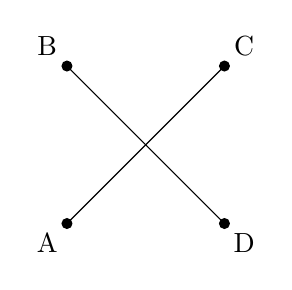
\begin{tikzpicture}
		\draw (0,0)--(2,2);
		\draw (0,2)--(2,0);
		\fill (0,0) circle(2pt);
		\fill (0,2) circle (2pt);
		\fill (2,2) circle (2pt);
		\fill (2,0) circle (2pt);
		\node at (-.25,-.25){A};
		\node at (-.25, 2.25){B};
		\node at (2.25, 2.25){C};
		\node at (2.25, -.25){D};
	\end{tikzpicture}
%%%%%%%%%%%%%%%%%%%%%%
%%%%%%%%%%%%%%%%%%%%%%%
	\item Moving to 3D, let us first think of the honeycomb cells as two layers of hexagonal prisms of equal heights, and the cell openings are on the top and the bottom. The wall in the middle of the two layers is not planar, and in fact it will take a shape that maintains the volume but minimizes the surface area, thus minimizing the wax required to make the hive. (This is mostly true.)\\
	\begin{multicols}{2}
	\begin{figure}[H]
		\includegraphics[scale=.45]{bees_a.png}
	\end{figure}
	\begin{figure}[H]
		\includegraphics[scale=.45]{bees_b.png}
	\end{figure}
	\end{multicols}
		\begin{enumerate}
			\item Let's walk through how to go from the left diagram to the right. First choose a distance, $y$, for $\overline{JN}$. Notice this defines a pyramid $JKIN$, rotate this pyramid 180$^\circ$ around the line $\overline{IK}$. This gives the rhombus $PKNI$ on the right. Explain why replacing the top base hexagon with 3 congruent rhombi preserves the volume of the honeycomb cell. Let's fix the volume of a cell by choosing $s$ constant as the sidelength of the hexagon and $h$ constant as the height of the hexagonal prism.
			\item Instead of $y$ as the parameter we vary, let's use the parameter $\theta$ to vary the shape of the honeycomb. It will be the angle between the vertical line through $P$ and one of the congruent rhombi. Express the area of one rhombus in terms of $\theta$. It will help to picture the pyramid $JKIN$ and that we started with regular hexagons as the base.
			\item Express the area of one of the trapezoidal lateral faces in terms of $\theta$. 
			\item Give the expression for the surface area of the cell, and takes its derivative with respect to $\theta$.
			\item What is the value of $\theta$ that minimizes the surface area? How do you know it is a minimum?			
		\end{enumerate}
	\item A possible extension is to look at the tetrahedral molecule Methane ($CH_4$). Show the angles of the bonds are related to the angles of the honeycomb.
	\item What other observations can you make? Feel free to research online at this point. What else might you be curious about?
	
	
		
\end{enumerate}

\newpage	    
    \section*{The Art Gallery Problem}
	\subsection*{Understanding the Problem}
We are given a gallery in the shape of an arbitrary $n$-sided polygon. The problem is to find the minimum number of guards needed to guarantee that every part of the gallery is in the line-of-sight of a guard without knowing the exact shape of the n-gon ahead of time. Let's define line-of-sight as points that can be connected to the guard with a line segment that stays within the polygon.
\begin{enumerate}
	\item  A good way to start this problem is to look at a few galleries and position guards, so that all of the gallery is within sight of a guard.
	\item  Notice for some polygons this problem is trivial, for instance how many guards do you need to watch a convex regular hexagon?
	\item However, other polygons can be a little more difficult to visualize. Try to find the minimum number of guards for the following 15-gon.
		\begin{figure}[H]
			\hspace{1cm} \includegraphics[scale=.3]{gall_a.png}
		\end{figure}
	\item Do you have a guess as to the minimum number of guards required to handle any $n$-gon.
		\end{enumerate}
\subsection*{A Possible Outline}
	\begin{enumerate}
		\item Prove any n-gon can be triangulated (cut into non-overlapping triangles) by connecting vertices. (be wary of concave polygons)
		\item Prove that once you have triangulated your polygon, you can 3-color the vertices, meaning assign 1 of 3 colors to each vertex such that no two connected vertices share a color. 
		\item Show that your 3-coloring of the polygon allows you to assign the minimal number of guards that will work for any n-gon.
	\end{enumerate}
	\newpage
\subsection*{A More Detailed Outline}
It will help to first show that any polygon can be triangulated. A polygon is triangulated when it is divided into triangles by drawing diagonals which are formed by connecting pairs of vertices. We will prove this by induction on the number of sides of the polygon.
	\begin{enumerate}
		\item Why is the base case $n=3$ true?
		\item The induction step here is a little tricky so we will break it into smaller steps.
			\begin{enumerate}
				\item First thinking about our $k+1$-gon, why must there be at least one convex ($<180^\circ$) vertex? 
				\item Label that convex vertex $Q$ and the adjacent vertices $P$ and $R$. If $\overline{PR}$ is a diagonal we are done. Explain.
				\item If $\overline{PR}$ is not a diagonal that means it must slip outside of the polygon, but then you can argue that there is a diagonal that has $Q$ as one of its endpoints. Explain. Use a diagram.
				
			\end{enumerate}
		\item Your proof that any polygon can be triangulated should be done. Look it over to make sure it makes sense and reads well.
	\end{enumerate}
	\vspace{1cm}
Now we will prove that for any $n$-gon, $\lfloor n/3 \rfloor$ guards will always be sufficient. First we will prove that any triangulation of a polygon can be 3-colored. For a triangulation to be 3-colored we mean the vertices of each triangle can be assigned a color 1, 2, or 3, so that no connected vertices are the same color.
\begin{enumerate}
	\item Prove by induction that any triangulation of an $n$-gon can be 3-colored.
	\item Suppose a guard is placed at the color that occurs least frequently. First explain why that gives $\lfloor n/3 \rfloor$ guards as the maximum number of guards. Then explain why this ensures all of the gallery is in view of a guard. 
	\item You're done! Write out your proof into one coherent argument. Read it one last time to make sure it reads well and makes sense. Be careful not to leave out key ideas.
\end{enumerate}
\newpage	    
    \section*{Getting to $\pi$ using Integration by Parts}
    In the following set of exercises you will derive an expression for $\pi$ that looks very appealing in its separation of odd and even integers.\\
    \begin{enumerate}
	\item Let $I_n =\displaystyle \int_0^\pi \sin^n(x)dx$. Use integration by parts to find a relationship between $I_n$ and $I_{n-2}$\\
	\item Calculuate $I_0$ and $I_1$.  Use this and the relationship you found inpart part a to find $I_k$ for $k=1, 2, 3, 4, 5, 6, 7$.  Don't simplify by multiplying. What patterns do you see?
	\item Make a guess for the formulas for $I_{2n}$ and $I_{2n+1}$. Make sure you get the indexing correct here, by checking against part b.
	\item Use mathematical induction to prove the equations for $I_{2n}$ and $I_{2n+1}$ that you guessed in part c. 
	\item Explain why $\sin^{2n+1}x \leq \sin^{2n}x \leq \sin^{2n-1} x$ for $x \in [0,\pi]$
	\item Explain why this gives the inequality $I_{2n+1} \leq I_{2n} \leq I_{2n-1}$
	\item Show that $\lim\limits_{n \to \infty} \dfrac{I_{2n}}{I_{2n+1}} =1$
	\item Show this gives a way to calculate $\dfrac{\pi}{2}$ as an infinite product. 
	\end{enumerate}

\newpage	    
    \section*{Predicting Peak Oil}
    
\newpage	    
    \section*{SIR: A Model for the Spread of Infectious Disease}

\newpage	    
    \section*{Modeling Air Resistance}

\newpage	    
    \section*{A Model for Combat}
	[Still working on it. Based upon Lanchester Laws]
\newpage	    
    \section*{A Model for Relationships}
	[Systems of Differential Equations. Still developing this one. May require matrices]
	\newpage
	
	\section*{Unbounded Integrals and $\sqrt{\pi}$}
	[The idea here is to show how one way to extend the factorial function to all real numbers involves integrating the logarithm from 0 to 1. Note it gives a value for gamme(1/2) I think as $\sqrt{\pi}$. 
	
	\newpage	    

%%%%%
%%%%%
%End of problems of the book.
%%%%%%%
%%%%%

\chapter{Answers}
\shipoutAnswer

\printbibliography

\end{document}
